\documentclass[a4paper, 11pt]{article}
\usepackage{comment} 
\usepackage{lipsum}  
\usepackage{fullpage} 

\usepackage[italian]{babel}
\selectlanguage{italian}
\usepackage[T1]{fontenc}
\usepackage[utf8]{inputenc}

\usepackage{graphicx}
\usepackage{hyperref}
\graphicspath{ {./images/} }

\begin{document}

%%%%%%%%%%%%%%%%%%%%%%%%%%%%%%%%%%%%%%%%%%%%%%%%%%%

\begin{titlepage}
	\centering
    \vspace*{0.5 cm}
    
\includegraphics[width=0.7\linewidth]{images/intercomsvg.png}\\[1.0 cm]
    \textsc{\LARGE Gestione Strategica delle Organizzazioni 18/19}\\[2.0 cm]
	\textsc{\Large Caso Unicorn}\\[0.5 cm]				
	\rule{\linewidth}{0.2 mm} \\[0.4 cm]
	{ \huge \bfseries Intercom}\\
	\rule{\linewidth}{0.2 mm} \\[1.5 cm]
	
	\begin{minipage}{0.4\textwidth}
		\begin{flushleft} \large
			Giovanni Candeo\\
		\end{flushleft}
		\end{minipage}~
		\begin{minipage}{0.4\textwidth}
            
		\begin{flushright} \large
            Matricola N. 1206150\\
		\end{flushright}
        
	\end{minipage}\\[2 cm]
	
\end{titlepage}

%%%%%%%%%%%%%%%%%%%%%%%%%%%%%%%%%%%%%%%%%%%%%%

\newpage
\noindent
\begin{minipage}{0.3\textwidth}

\includegraphics[width=0.75 \linewidth]{images/intercomlogo.png}
\end{minipage}
\hfill
\begin{minipage}{0.7\textwidth}\raggedleft
Azienda: Intercom\\
Location: San Francisco, California, United States \\
Anno di costituzione: 2011 \\
Data di ingresso nella lista Unicorn: 7/3/2018 \\
Settore Principale: Internet \& Customer Relation Management
\end{minipage}\\
\par\noindent\rule{\textwidth}{0.4pt}

\section*{Il problema da risolvere}
L'avvento del Web ha portato ad un cambiamento delle relazioni con i clienti da parte delle imprese, ora in grado di offrire servizi tramite siti Web e applicazioni affini.\\
L'evoluzione e innovazione nel campo che viene chiamato CRM (Customer Relationship Management) diventa quindi una necessità. \\
In un intervista, Eoghan McCabe, CEO di Intercom, rimarca il problema:\\ \par
\textit{“Businesses don't know or talk to the people who use their products and customers don’t know or talk to the people who make products.  While businesses have tools to run online help desks, email marketing, customer relationship management and marketing automation, [...] they cannot provide a holistic view of the customer. As a result, the customer’s experience is very disjointed. \cite{Pamela}”}
\\
\\
Nel campo CRM, Intercom si è posta vari problemi da risolvere, alcuni esempi sono: la natura impersonale dei messaggi ai clienti, lo scarso \textit{targeting} e tempistica di tali messaggi, la mancanza del contesto, il fatto che tali messaggi non siano molto colloquiali, e il fatto che molti di questi strumenti considerino il Web e il mobile come due cose separate \cite{tc1}.

\section*{Concept di prodotto/servizio}
\par 
Il \emph{core product} di \textit{Intercom} è un applicazione di assistenza clienti che gestisce e integra tutti i modi in cui le aziende comunicano con i loro clienti, ciò comprende ad esempio una piattaforma di messaggistica che consente la comunicazione all'interno della loro \textit{app}, sul loro sito web, attraverso i \textit{social media} o via email.\\
Oltre a questo, \textit{Intercom} fornisce la possibilità di tracciare i dati relativi ai clienti, fornendo quindi alle imprese strumenti utili anche per l'analisi dei clienti.\\
Il concept è quello di fornire un servizio unico a 360 gradi per qualunque esigenza nel campo CRM per ogni tipo di azienda.\par
\section*{Tecnologie adottate}
Intercom fornisce un prodotto che necessita di essere trasversale nell'ambito del Web e del mobile, campi in continua evoluzione nella tecnologia.\\
L'innovazione in ambito tecnologico per Intercom significa quindi l'adozione di nuovi frameworks e lo sfruttamento al 100\% della programmazione Ajax e di linguaggi come il JavaScript. (vedi figura \ref{fig:tecnologie} per l'intero \textit{Tech Stack})

\section*{Stima del mercato di riferimento}

\emph{"As ‘software eats the world’, in the words of Netscape’s Marc Andreessen, all businesses are becoming web businesses. The potential for these businesses to sell to and support customers at scale is truly awesome"  \cite{Pamela}}\\
\null \hfill Eoghan McCabe, Intercom CEO.
\subsection*{\textit{Segmentazione del mercato}}
\par
Il mercato della CRM si può suddividere in quattro livelli\cite{GVR}: distribuzione, utilizzo finale, applicazione e area geografica (vedi figura \ref{fig:segmentationintercom}).\\
Nel primo livello, il mercato si può segmentare per implementazione in sede e implementazione in \textit{cloud}. 
L'implementazione in sede implica l'\textit{hosting} della suite CRM sui server dell'azienda e viene generalmente preferito dalle aziende che vogliono memorizzare informazioni riservate nei loro server piuttosto che in \textit{cloud}.\\
Il secondo livello, utilizzo finale, viene suddiviso in base alla dimensione dell'azienda, quindi grandi e piccole-medie imprese.\\
Il terzo livello fa riferimento all'area di applicazione di un applicativo CRM, quindi aree quali: \textit{BFSI} (servizi bancari, finanziari e assicurativi), vendita al dettaglio, assistenza sanitaria, telecomunicazioni e \textit{Information Technology}, \textit{Discrete Manifacturing}, governo ed educazione.\\
Il quarto livello suddivide il mercato in base all'area geografica: America del Nord, Europa, Asia e Pacifico, America latina, \textit{MEA} (regioni del Medio Oriente e Africa).

\subsection*{\textit{Dimensioni del mercato e prospettive di crescita}}
\par 
Le dimensioni del mercato globale del Customer Relationship Management (CRM) sono state valutate di 23,14 miliardi di dollari nel 2015 e secondo un report di \textit{Grand View Research, Inc}, il mercato globale della \textit{Customer Relationship Management} dovrebbe raggiungere gli 81,9 miliardi di dollari di valore entro il 2025 \cite{GVR}  (vedi figura \ref{fig:crescitacrm}). \\
Le soluzioni per la gestione della relazioni con i clienti hanno subito un forte aumento di crescita e di numero di adozioni negli ultimi anni nonostante la presenza nel mercato da oltre 20 anni. La crescita di questo \textit{trend} è prevista per gli anni a venire dal momento che le imprese, grandi e piccole, hanno compreso i benefici di una \textit{suite} CRM in grado di ridurre i costi operativi, i costi del marketing e la capacità di completare cicli di vendita "al volo". 

\subsection*{\textit{Concorrenza nel mercato}}
\par
La concorrenza sul mercato è alta con pochi venditori come \textit{Salesforce}, \textit{Microsoft}, \textit{Oracle} e \textit{SAP} che riforniscono quasi la metà del mercato. Nonostante ciò, alcuni piccoli operatori (start-up come Intercom e operatori regionali) stanno tagliando la quota di mercato di questi venditori. I "giocatori" del settore praticano un alto grado di innovazione e personalizzazione per fornire soluzioni uniche ai clienti esistenti e potenziali. Acquisizioni e fusioni sono anche dilaganti nel settore, in particolare per l'ampliamento del portfolio dei prodotti delle aziende.\cite{GVR} \\(vedi il modello di Porter nella figura \ref{fig:porterintercom})\\

\newpage\section*{Profilo dell’utente primario e degli altri (potenziali) utenti}
Intercom si propone a qualunque tipo di azienda, grande o piccola, tramite un servizio scalabile per dimensioni di azienda e necessità: acquisizione, coinvolgimento e assistenza clienti.\\
L'utente primario tuttavia è una start-up o un'azienda medio-piccola/start-up che offre un servizio online o possiede un portale web per la vendita di prodotti.\\

\section*{Analisi dei competitor e differenziazione}

\emph{“Minimizing customer interaction is a very outdated model from a pre-social web world. Intercom is very much about intimacy, very much about being personable.” \cite{tc2}} \\
\null \hfill Paul Adams, VP di produzione ad \textit{Intercom}\\ 
\par
Mentre nel passato si cercava di minimizzare le interazioni con il cliente, \textit{Intercom} propone un nuovo approccio, cercando di portare le "relazioni umane" su Internet.\\
Questa tipo d'approccio e una politica d'impresa innovativa orientata al cliente è il fattore principale che ha portato l'azienda a ritagliarsi uno \textit{sweet spot} nel mercato dei software per il CRM, un settore denso di \textit{competitor} come \textit{Braze}, \textit{Marketo}, \textit{Drift}, \textit{iAdvize}, \textit{Nimble}, \textit{InsideView} e \textit{RelatelQ}.\\
Un altro fattore che contribuisce alla differenziazione di \textit{Intercom} rispetto alle altre aziende nel settore è la capacità di fornire un prodotto scalabile ma uniforme in grado di soddisfare ogni tipo di esigenza per ogni tipo e scala di business.


\section*{Modello di business e fonti di ricavo}
\par
Intercom focalizza il suo modello di business sulla differenziazione del proprio prodotto rispetto ai competitors. Nel corso degli anni ha dimostrato di fornire un prodotto di qualità e innovativo grazie soprattutto alla sua politica d'impresa "\textit{product-first and product-oriented}" e un particolare \textit{focus} sul proprio reparto di ricerca e sviluppo che costituisce la metà dell'organico dell'azienda.\cite{tc3}\\

Attraverso il proprio sito web, \textit{intercom.com}, da la possibilità a chiunque azienda di beneficiare dei servizi di CRM che vengono messi a disposizione tramite un abbonamento mensile con prezzo variabile in base al piano richiesto.\\
Intercom fornisce anche un \textit{free-trial} di 14 giorni, offrendo quindi maggiore flessibilità e accessibilità economica ai nuovi utenti e favorendo maggiori profitti nel lungo termine.\\
Importante nota è anche la possibilità di integrare i servizi Intercom con altri quali: \textit{Stripe, Hubspot, Shopify, Salesforce, Zendesk, Github}; ciò contribuisce alla creazione di un effetto \textit{network} e conseguente aumento del valore di \textit{business}.\\

\newpage
\section*{Profilo dei Founders}
\par Intercom è nata nel 2011 dalle menti di Eoghan McCabe, Des Traynor, Ciaran Lee e David Barrett, ingegneri e designers irlandesi che avevano l'abitudine di ritrovarsi in un coffee shop a Dublino chiamato \textit{Third Floor Espresso.}\\
Lavorano insieme già da qualche anno in \textit{Contrast}, un azienda di consulenza per il design del software, e durante le svariate ore spese nel locale non possono fare altro che notare quanto le relazioni fra il proprietario del locale e i suoi clienti siano diverse rispetto a quelle nel loro lavoro.\\
L'interazione che il proprietario del coffee shop aveva con la gente che sedeva al bancone gli permetteva di sviluppare un "vero" rapporto umano e di fidelizzazione.\\
Realizzano quindi che uno dei veri problemi del business sul web è questo: le aziende raramente incontrano i loro clienti, non c'è la creazione di una relazione "umana" che si crea ad esempio nel momento in cui si ordina da bere al bancone di un bar.\\
Al tempo erano già presenti molti software o suite CRM ma pochi si focalizzavano sull’aspetto della creazione di una relazione "umana" con il cliente.\\
Per quanto banale possa sembrare un idea di questo tipo, i quattro irlandesi si misero al lavoro per risolvere proprio questo problema di comunicazione tra business e uomo, con la forte convinzione che le relazioni di questo tipo siano indispensabili per migliorare le imprese.

\section*{Investimenti ottenuti}
\par Intercom fu fondata nel 2011 grazie ai profitti ottenuti della vendita di \textit{Exceptional}, start-up fondata sempre da McCabe, Traynor, Lee e Barret, di cui erano propietari.\\
Nel 2012, a seguito di un investimento di una somma non rivelata da parte del co-fondatore di \textit{Twitter} Biz Stone\cite{bi}, l'azienda si porta sotto i riflettori del mercato delle start-up ed inizia ad attrarre finanziamenti rilevanti da parte di nomi quali David Sacks, Andy McLoughlin (fondatore di \textit{Huddle}), Dan Martell (fondatore \textit{Flowtown}) e Dave McClure (\textit{500 Startups})\cite{inv}.\\
Nel corso degli anni riceve altri investimenti importanti come un finanziamento di Serie A da \$ 6 milioni nel 2013 da parte di \textit{Social Capital}, un finanziamento di \$ 23 milioni in serie B da parte di \textit{Bessemer Venture Partners} nel gennaio 2014 e un finanziamento di \$ 50 milioni in serie C-1 da \textit{Index Ventures} nel 2016.
Nel 2018 inoltre Intercom ha annunciato un round di Serie D da \$ 125 milioni guidato da Kleiner Perkins, con la partecipazione di \textit{Google Ventures}. (vedi figura \ref{fig:investimenti} investimenti per maggiori dettagli).

\section*{Prospettive di crescita dell’impresa}
\par Intercom ha raggiunto lo status di \textit{unicorn} all'inizio del 2018 dopo aver raccolto \$ 125 milioni per portare la sua valutazione a oltre \$ 1 miliardo; nonostante ciò non è stata in grado di ridurre le perdite, invariate a \$ 22,4 milioni. Resta comunque inteso che le perdite per l'intero anno sono dovute in gran parte agli investimenti da parte dell'azienda nell'attività di ricerca e sviluppo.
I conti registrati di recente per il fatturato di \textit{Intercom R\&D Unlimited Company} per 12 mesi a partire da gennaio 2018 sono passati da \$ 33,1 milioni a \$ 61,5 milioni a seguito della crescita dei ricavi medi per cliente del 28,6\%.\\
Intercom al momento conta più di 30.000 clienti per i suoi servizi tra cui \textit{Sotheby's}, \textit{Spotify}, \textit{New Relic} e \textit{Shopify} e sembra puntare sempre di più sull'intelligenza artifiale; la compagnia di recente ha lanciato il suo primo chatbot autonomo conosciuto come \textit{AnswerBot}: un bot guidato da un intelligenza artificiale che usa tecnologie di machine learning per rispondere alle domande del cliente.\cite{irishtimes}
\newpage 

% \section*{Tabelle}
% \begin{table}[h]
% \begin{center}
% \begin{tabular}{ |p{5cm}|p{10cm}| } 
% \hline
% Databases &	Mongodb, Mysql, Redis \\ \hline
% Frameworks/Libraries &	Ajax, Boost, Ember.Js, Hadoop, Node.Js, Prototype, Sinatra, Solr, Tactic, Wordpress \\\hline
% Infrastructure & Aws, Heroku, Rackspace \\\hline
% Operating Systems &	Android, Ios, Windows \\\hline
% Programming Languages &	Asp, Assembly, Go, Io, Java, Javascript, Matlab, Perl, Php, Processing, Python, R, Ruby, Scala, Scheme \\\hline
% Server/Network & Elasticsearch, Https, Nginx, Soap \\\hline
% Software Applications &	Github, Outlook, Salesforce, Sas \\\hline
% Other &	Amazon, Animation, Api, Apple, Architecture, Arm, Asynchronous, Audio, Automation, Backup, Browser, Calendar, Charts, Console, Css, Gmail, Hardware, Html, Icons, Microsoft, Migration, Mobile, Numbers, Optimization, Positioning, Protocols, Push, Replication, Scale, Sql, Stack, Storage, Testing, Twitter, Website \\
%  \hline
% \end{tabular}
% \caption{Tabella delle tecnologie adottate.}
% \label{table:1}
% \end{center}
% \end{table}

\newpage
\section*{Figure}
\null
\vfill
\begin{figure}[h]
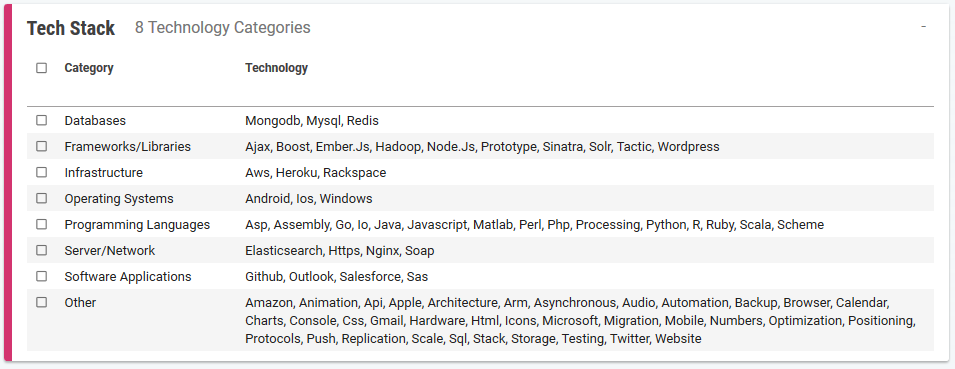
\includegraphics[width=\textwidth]{images/intercomTech.PNG}
\caption{Tabella delle tecnologie adottate.}
\label{fig:tecnologie}
\end{figure}
\begin{figure}[h]
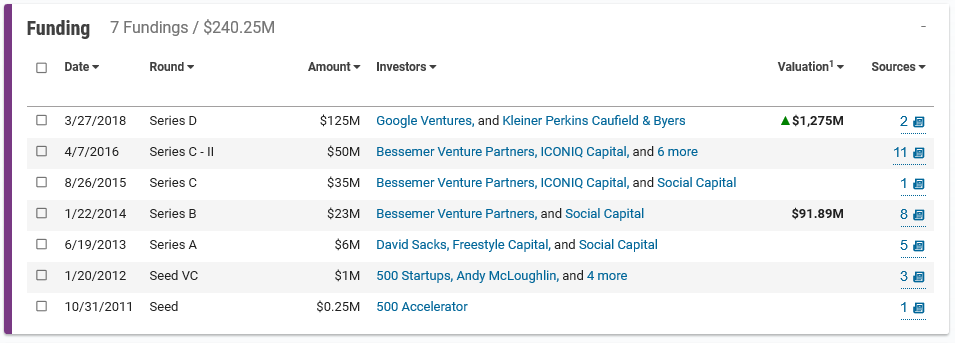
\includegraphics[width=\textwidth]{images/intercomFundings.PNG}
\caption{Tabella dei finanziamenti di Intercom}
\label{fig:investimenti}
\end{figure}
\vfill

\newpage
\null
\vfill
\begin{figure}[h]
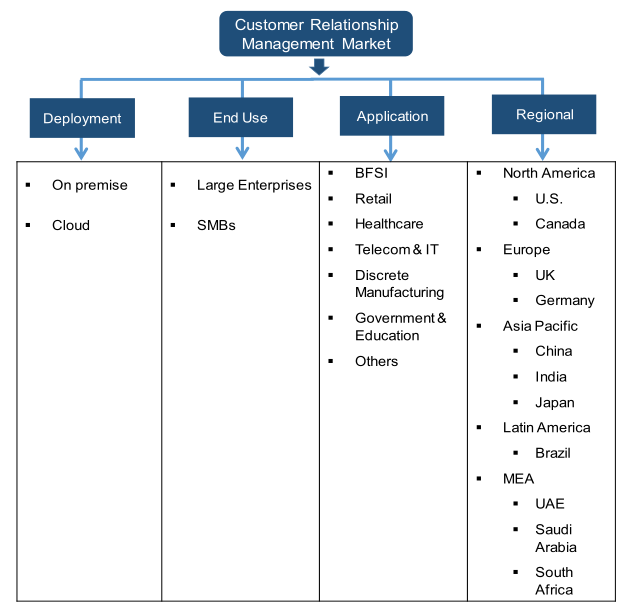
\includegraphics[width=\textwidth]{images/CRMmarketsegmentation.PNG}
\caption{Segmentazione del mercato CRM  \cite{GVR}}
\label{fig:segmentationintercom}
\end{figure}
\vfill

\newpage
\null
\vfill
\begin{figure}[h]
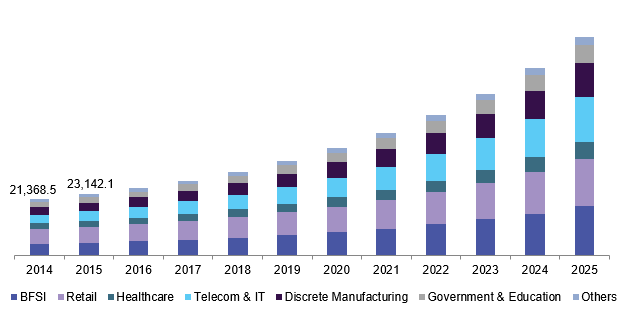
\includegraphics[width=\textwidth]{images/global-customer-relationship-management-market.png}
\caption{Mercato globale della \textit{Customer Relationship Management}, per area di applicazione, 2014 - 2025 (milioni di dollari) \cite{GVR}}
\label{fig:crescitacrm}
\end{figure}
\vfill

\newpage
\null
\vfill
\begin{figure}[h]
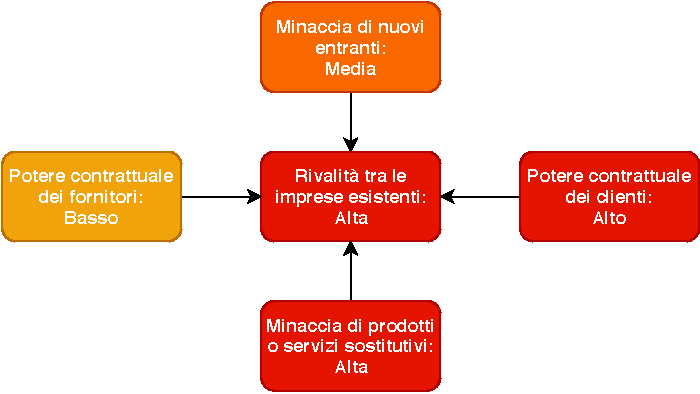
\includegraphics[width=\textwidth]{images/porterintercom.pdf}
\caption{Modello delle cinque forze competitive di Porter per il mercato CRM \cite{GVR}}
\label{fig:porterintercom}
\end{figure}
\vfill

\newpage
\section*{Note}
Informazioni principali dell'azienda ottenute grazie anche a \href{www.wikipedia.org}{Wikipedia}.\\
Aziende \textit{competitor} ottenute dal profilo dell'azienda su \href{www.cbinsights.com}{\textit{CB Insights}}.\\
Tabella delle tecnologie adottate ottenute dal profilo dell'azienda su  \href{www.cbinsights.com}{\textit{CB Insights}}.\\
Il codice sorgente LaTeX utilizzato per creare questo report è disponibile nella \href{https://github.com/candeogi/HomeworkGSO}{repository GitHub}.\\

\begin{thebibliography}{9}
\bibitem{Pamela}
Newenham, Pamela. \emph{"Four Irishmen on a mission to build a billion-dollar company"}. \emph{The Irish Times}. 23 Gennaio 2014.
\bibitem{tc1} Ha, Anthony. \emph{"With Intercom’s New In-App Messenger, Businesses Can Get Smarter About Talking To Customers"}. \emph{TechCrunch}. 4 Settembre 2014.
\bibitem{tc2}Ha, Anthony. \emph{"Facebook’s Head Of Brand Design Paul Adams Joins Customer Outreach Startup Intercom"}.\emph{TechCrunch}. 24 Maggio 2013.
\bibitem{GVR} \textit{"Customer Relationship Management (CRM) Market Analysis By Deployment, By Enterprise Size, By Application (BFSI, Retail, Healthcare, Telecom \& IT, Discrete Manufacturing), By Region, And Segment Forecasts, 2018 - 2025"}. \textit{Grand View Research}. Aprile 2017.
\bibitem{bi} Bort, Julie. \textit{"How drinking Guinness with Biz Stone launched one of the fastest-growing startups in the Valley today"}. \textit{Business Insider}. 22 Febbraio 2017.
\bibitem{inv} O'Dell, Jolie. \textit{"Startup Intercom nabs \$1M from Biz Stone and other prominent angels"}. \textit{Reuters}. 25 January 2012.
\bibitem{tc3} Ha, Anthony. \emph{"Intercom Raises \$35M To Make Businesses Smarter About Their Customer Communication"}. \emph{TechCrunch}. 26 Agosto 2015.
\bibitem{irishtimes} Taylor, Charlie. \textit{Revenues almost double at Irish tech company Intercom}. \textit{The Irish Times}. 19 Dicembre 2018.
\end{thebibliography}

\end{document}
